\pdfminorversion=4
\documentclass[aspectratio=169]{beamer}

\mode<presentation>
{
  \usetheme{default}
  \usecolortheme{default}
  \usefonttheme{default}
  \setbeamertemplate{navigation symbols}{}
  \setbeamertemplate{caption}[numbered]
  \setbeamertemplate{footline}[frame number]  % or "page number"
  \setbeamercolor{frametitle}{fg=white}
  \setbeamercolor{footline}{fg=black}
} 

\usepackage[english]{babel}
\usepackage[utf8x]{inputenc}
\usepackage{tikz}
\usepackage{courier}
\usepackage{array}
\usepackage{bold-extra}
\usepackage{minted}
\usepackage[thicklines]{cancel}
\usepackage{fancyvrb}

\xdefinecolor{dianablue}{rgb}{0.18,0.24,0.31}
\xdefinecolor{darkblue}{rgb}{0.1,0.1,0.7}
\xdefinecolor{darkgreen}{rgb}{0,0.5,0}
\xdefinecolor{darkgrey}{rgb}{0.35,0.35,0.35}
\xdefinecolor{darkorange}{rgb}{0.8,0.5,0}
\xdefinecolor{darkred}{rgb}{0.7,0,0}
\definecolor{darkgreen}{rgb}{0,0.6,0}
\definecolor{mauve}{rgb}{0.58,0,0.82}

\title[2019-10-17-pyhep-awkward]{Uproot and Awkward-Array in the Year of Python}
\author{Jim Pivarski}
\institute{Princeton University -- IRIS-HEP}
\date{October 17, 2019}

\usetikzlibrary{shapes.callouts}

\begin{document}

\logo{\pgfputat{\pgfxy(0.11, 7.4)}{\pgfbox[right,base]{\tikz{\filldraw[fill=dianablue, draw=none] (0 cm, 0 cm) rectangle (50 cm, 1 cm);}\mbox{\hspace{-8 cm}\includegraphics[height=1 cm]{princeton-logo-long.png}\hspace{0.1 cm}\raisebox{0.1 cm}{\includegraphics[height=0.8 cm]{iris-hep-logo-long.png}}\hspace{0.1 cm}}}}}

\begin{frame}
  \titlepage
\end{frame}

\logo{\pgfputat{\pgfxy(0.11, 7.4)}{\pgfbox[right,base]{\tikz{\filldraw[fill=dianablue, draw=none] (0 cm, 0 cm) rectangle (50 cm, 1 cm);}\mbox{\hspace{-8 cm}\includegraphics[height=1 cm]{princeton-logo.png}\hspace{0.1 cm}\raisebox{0.1 cm}{\includegraphics[height=0.8 cm]{iris-hep-logo.png}}\hspace{0.1 cm}}}}}

% Uncomment these lines for an automatically generated outline.
%\begin{frame}{Outline}
%  \tableofcontents
%\end{frame}

% START START START START START START START START START START START START START

\begin{frame}{}
\LARGE
\vspace{1 cm}
\begin{center}
\textcolor{darkblue}{Year of Python?}
\end{center}
\end{frame}

\begin{frame}{On Scientific Linux, uproot/awkward is installed as often as Pandas}
\vspace{0.5 cm}
\begin{columns}
\column{1.2\linewidth}
\includegraphics[width=\linewidth]{pip-scilinux-uproot.pdf}
\end{columns}
\end{frame}

\begin{frame}{And so is Coffea\ldots}
\vspace{0.5 cm}
\begin{columns}
\column{1.2\linewidth}
\includegraphics[width=\linewidth]{pip-scilinux-uproot-iminuit.pdf}
\end{columns}
\end{frame}

\begin{frame}{\ldots more so than deep learning libraries (TensorFlow and Torch)}
\vspace{0.5 cm}
\begin{columns}
\column{1.2\linewidth}
\includegraphics[width=\linewidth]{pip-scilinux-ml.pdf}
\end{columns}
\end{frame}

\begin{frame}{But take a step back and look in linear scale!}
\vspace{0.5 cm}
\begin{columns}
\column{1.2\linewidth}
\includegraphics[width=\linewidth]{pip-scilinux-linear.pdf}
\end{columns}
\end{frame}

\begin{frame}{The bigger news is that more physicists are using Python {\it this year}}
\vspace{0.5 cm}
\begin{columns}
\column{1.2\linewidth}
\includegraphics[width=\linewidth]{pip-scilinux-everything.pdf}
\end{columns}
\end{frame}

\begin{frame}{(In general, uproot is 4 orders of magnitude from Pandas)}
\vspace{0.5 cm}
\begin{columns}
\column{1.2\linewidth}
\only<1>{\includegraphics[width=\linewidth]{pip-linux.pdf}}\only<2>{\includegraphics[width=\linewidth]{pip-macos.pdf}}\only<3>{\includegraphics[width=\linewidth]{pip-windows.pdf}}
\end{columns}
\end{frame}

\begin{frame}{Another way to see Python usage among physicists: GitHub repos}
\begin{columns}
\column{1.2\linewidth}
\only<1>{\includegraphics[width=\linewidth]{github-linear.pdf}}\only<2>{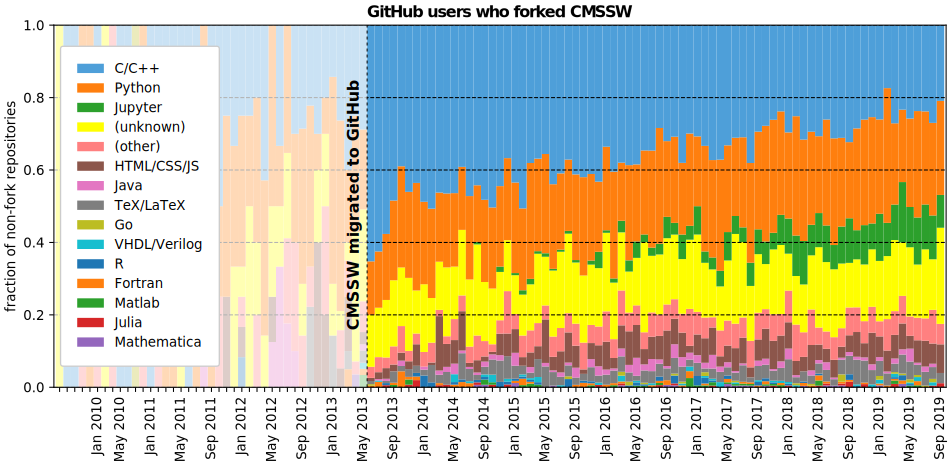
\includegraphics[width=\linewidth]{github-fraction.pdf}}\only<3>{\includegraphics[width=\linewidth]{github-simplefraction.pdf}}
\end{columns}
\end{frame}

\begin{frame}{Maintainance is pretty much constant}
\vspace{0.5 cm}
\begin{columns}
\column{0.36\linewidth}
\includegraphics[width=\linewidth]{uproot-issues.pdf}

\column{0.72\linewidth}
\only<1>{\includegraphics[width=0.5\linewidth]{uproot-users.pdf}\hfill\includegraphics[width=0.5\linewidth]{uproot-comments.pdf}}\only<2>{\centering \includegraphics[width=0.45\linewidth]{uproot-response-time.pdf}}
\end{columns}
\end{frame}


\end{document}
